\chapter{DNA replication}\label{dna-replication}

In molecular biology, DNA replication is the biological process of producing two identical replicas of DNA from one original DNA molecule. DNA replication occurs in all living organisms acting as the basis for biological inheritance. The cell possesses the distinctive property of division, which makes replication of DNA essential.

DNA is made up of a double helix of two complementary strands. During replication, these strands are separated. Each strand of the original DNA molecule then serves as a template for the production of its counterpart, a process referred to as semiconservative replication. As a result of semi-conservative replication, the new helix will be composed of an original DNA strand as well as a newly synthesized strand. Cellular proofreading and error-checking mechanisms ensure near perfect fidelity for DNA replication.



\begin{figure}

{\centering 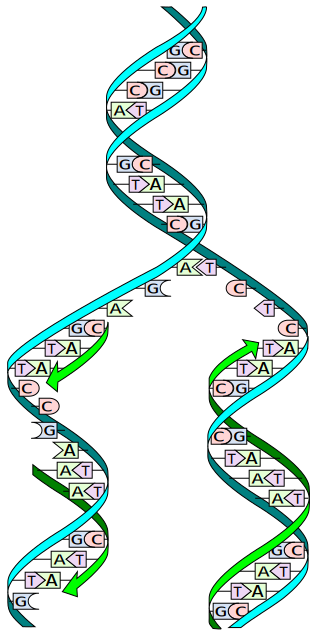
\includegraphics[width=0.7\linewidth]{./figures/replication/DNA_replication_split} 

}

\caption{\href{https://commons.wikimedia.org/wiki/File:DNA_replication_split.svg}{DNA polymerases adds nucleotides to the 3′ end of a strand of DNA. If a mismatch is accidentally incorporated, the polymerase is inhibited from further extension. Proofreading removes the mismatched nucleotide and extension continues.}}\label{fig:repfork}
\end{figure}

In a cell, DNA replication begins at specific locations, or origins of replication, in the genome. Unwinding of DNA at the origin and synthesis of new strands, accommodated by an enzyme known as helicase, results in replication forks growing bi-directionally from the origin. A number of proteins are associated with the replication fork to help in the initiation and continuation of DNA synthesis. Most prominently, DNA polymerase synthesizes the new strands by adding nucleotides that complement each (template) strand. DNA replication occurs during the S-stage of interphase.

DNA replication (DNA amplification) can also be performed in vitro (artificially, outside a cell). DNA polymerases isolated from cells and artificial DNA primers can be used to start DNA synthesis at known sequences in a template DNA molecule. Polymerase chain reaction (PCR), ligase chain reaction (LCR), and transcription-mediated amplification (TMA) are examples.

\hypertarget{eukaryotic-dna-replication}{%
\section{Eukaryotic DNA replication}\label{eukaryotic-dna-replication}}

Eukaryotic DNA replication is a conserved mechanism that restricts DNA replication to once per cell cycle. Eukaryotic DNA replication of chromosomal DNA is central for the duplication of a cell and is necessary for the maintenance of the eukaryotic genome.

DNA replication is the action of DNA polymerases synthesizing a DNA strand complementary to the original template strand. To synthesize DNA, the double-stranded DNA is unwound by DNA helicases ahead of polymerases, forming a replication fork containing two single-stranded templates. Replication processes permit the copying of a single DNA double helix into two DNA helices, which are divided into the daughter cells at mitosis. The major enzymatic functions carried out at the replication fork are well conserved from prokaryotes to eukaryotes, but the replication machinery in eukaryotic DNA replication is a much larger complex, coordinating many proteins at the site of replication, forming the replisome.

After the replicative helicase has unwound the parental DNA duplex, exposing two single-stranded DNA templates, replicative polymerases are needed to generate two copies of the parental genome. DNA polymerase function is highly specialized and accomplish replication on specific templates and in narrow localizations. At the eukaryotic replication fork, there are three distinct replicative polymerase complexes that contribute to DNA replication: Polymerase α, Polymerase δ, and Polymerase ε. These three polymerases are essential for viability of the cell.



\begin{figure}

{\centering 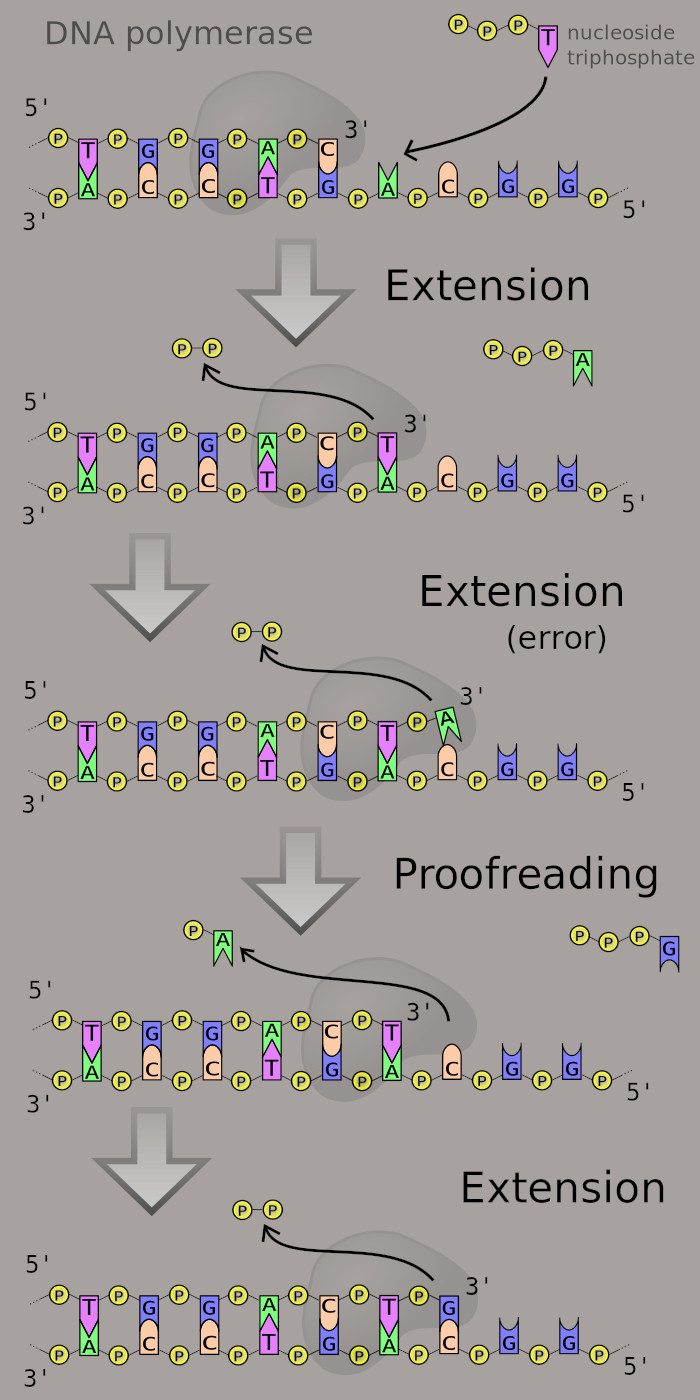
\includegraphics[width=0.7\linewidth]{./figures/replication/DNA_polymerase} 

}

\caption{\href{https://commons.wikimedia.org/wiki/File:DNA_polymerase.svg}{DNA polymerases adds nucleotides to the 3′ end of a strand of DNA. If a mismatch is accidentally incorporated, the polymerase is inhibited from further extension. Proofreading removes the mismatched nucleotide and extension continues.}}\label{fig:polymerase}
\end{figure}

Because DNA polymerases require a primer on which to begin DNA synthess, polymerase α (Pol α) acts as a replicative primase. Pol α is associated with an RNA primase and this complex accomplishes the priming task by synthesizing a primer that contains a short 10 nucleotide stretch of RNA followed by 10 to 20 DNA bases. Importantly, this priming action occurs at replication initiation at origins to begin leading-strand synthesis and also at the 5' end of each Okazaki fragment on the lagging strand.

However, Pol α is not able to continue DNA replication and must be replaced with another polymerase to continue DNA synthesis. Polymerase switching requires clamp loaders and it has been proven that normal DNA replication requires the coordinated actions of all three DNA polymerases: Pol α for priming synthesis, Pol ε for leading-strand replication, and the Pol δ, which is constantly loaded, for generating Okazaki fragments during lagging-strand synthesis.

\begin{itemize}
\tightlist
\item
  Polymerase α (Pol α): Forms a complex with a small catalytic subunit (PriS) and a large noncatalytic (PriL) subunit. First, synthesis of an RNA primer allows DNA synthesis by DNA polymerase alpha. Occurs once at the origin on the leading strand and at the start of each Okazaki fragment on the lagging strand. Pri subunits act as a primase, synthesizing an RNA primer. DNA Pol α elongates the newly formed primer with DNA nucleotides. After around 20 nucleotides, elongation is taken over by Pol ε on the leading strand and Pol δ on the lagging strand.
\item
  Polymerase δ (Pol δ): Highly processive and has proofreading, 3'-\textgreater{}5' exonuclease activity. In vivo, it is the main polymerase involved in both lagging strand and leading strand synthesis.
\item
  Polymerase ε (Pol ε): Highly processive and has proofreading, 3'-\textgreater{}5' exonuclease activity. Highly related to pol δ, in vivo it functions mainly in error checking of pol δ.
\end{itemize}

The replisome is responsible for copying the entirety of genomic DNA in each proliferative cell. This process allows for the high-fidelity passage of hereditary/genetic information from parental cell to daughter cell and is thus essential to all organisms. Much of the cell cycle is built around ensuring that DNA replication occurs without errors.



\begin{figure}

{\centering 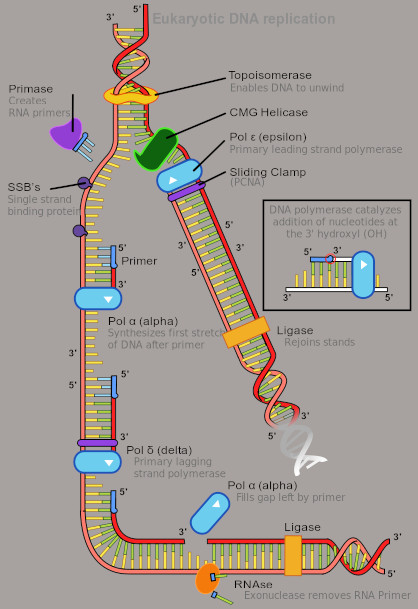
\includegraphics[width=0.7\linewidth]{./figures/replication/Eukaryotic_DNA_replication} 

}

\caption{\href{https://commons.wikimedia.org/wiki/File:Eukaryotic_DNA_replication.svg}{Many enzymes are involved in forming the DNA replication fork and DNA polymerization.}}\label{fig:repforkform}
\end{figure}

In G1 phase of the cell cycle, many of the DNA replication regulatory processes are initiated. In eukaryotes, the vast majority of DNA synthesis occurs during S phase of the cell cycle, and the entire genome must be unwound and duplicated to form two daughter copies. During G2, any damaged DNA or replication errors are corrected. Finally, one copy of the genomes is segregated to each daughter cell at mitosis or M phase. These daughter copies each contain one strand from the parental duplex DNA and one nascent antiparallel strand.

This mechanism is conserved from prokaryotes to eukaryotes and is known as semiconservative DNA replication. The process of semiconservative replication for the site of DNA replication is a fork-like DNA structure, the replication fork, where the DNA helix is open, or unwound, exposing unpaired DNA nucleotides for recognition and base pairing for the incorporation of free nucleotides into double-stranded DNA.

DNA replication, like all biological polymerization processes, proceeds in three enzymatically catalyzed and coordinated steps: initiation, elongation and termination.

\hypertarget{initiation}{%
\subsection{Initiation}\label{initiation}}

For a cell to divide, it must first replicate its DNA. DNA replication is an all-or-none process; once replication begins, it proceeds to completion. Once replication is complete, it does not occur again in the same cell cycle. This is made possible by the division of initiation into two temporally distinct steps: formation of the pre-replication complex and the preinitiation complex.

\hypertarget{pre-replication-complex}{%
\subsection{Pre-replication complex}\label{pre-replication-complex}}

In late mitosis and early G1 phase, a large complex of initiator proteins assembles into the pre-replication complex at particular points in the DNA, known as ``origins''. In E. coli the primary initiator protein is DnaA; in yeast, this is the origin recognition complex. Sequences used by initiator proteins tend to be ``AT-rich'' (rich in adenine and thymine bases), because A-T base pairs have two hydrogen bonds (rather than the three formed in a C-G pair) and thus are easier to strand-separate. In eukaryotes, the origin recognition complex catalyzes the assembly of initiator proteins into the pre-replication complex. Cdc6 and Cdt1 then associate with the bound origin recognition complex at the origin in order to form a larger complex necessary to load the Mcm complex onto the DNA. The Mcm complex is the helicase that will unravel the DNA helix at the replication origins and replication forks in eukaryotes. The Mcm complex is recruited at late G1 phase and loaded by the ORC-Cdc6-Cdt1 complex onto the DNA via ATP-dependent protein remodeling. The loading of the Mcm complex onto the origin DNA marks the completion of pre-replication complex formation.

If environmental conditions are right in late G1 phase, the G1 and G1/S cyclin-Cdk complexes are activated, which stimulate expression of genes that encode components of the DNA synthetic machinery. G1/S-Cdk activation also promotes the expression and activation of S-Cdk complexes, which may play a role in activating replication origins depending on species and cell type. Control of these Cdks vary depending cell type and stage of development. This regulation is best understood in budding yeast, where the S cyclins Clb5 and Clb6 are primarily responsible for DNA replication. Clb5,6-Cdk1 complexes directly trigger the activation of replication origins and are therefore required throughout S phase to directly activate each origin.

In a similar manner, Cdc7 is also required through S phase to activate replication origins. Cdc7 is not active throughout the cell cycle, and its activation is strictly timed to avoid premature initiation of DNA replication. In late G1, Cdc7 activity rises abruptly as a result of association with the regulatory subunit Dbf4, which binds Cdc7 directly and promotes its protein kinase activity. Cdc7 has been found to be a rate-limiting regulator of origin activity. Together, the G1/S-Cdks and/or S-Cdks and Cdc7 collaborate to directly activate the replication origins, leading to initiation of DNA synthesis.

\hypertarget{preinitiation-complex}{%
\subsection{Preinitiation complex}\label{preinitiation-complex}}

In early S phase, S-Cdk and Cdc7 activation lead to the assembly of the preinitiation complex, a massive protein complex formed at the origin. Formation of the preinitiation complex displaces Cdc6 and Cdt1 from the origin replication complex, inactivating and disassembling the pre-replication complex. Loading the preinitiation complex onto the origin activates the Mcm helicase, causing unwinding of the DNA helix. The preinitiation complex also loads α-primase and other DNA polymerases onto the DNA.

After α-primase synthesizes the first primers, the primer-template junctions interact with the clamp loader, which loads the sliding clamp onto the DNA to begin DNA synthesis. The components of the preinitiation complex remain associated with replication forks as they move out from the origin.

\hypertarget{elongation}{%
\subsection{Elongation}\label{elongation}}

DNA polymerase has 5′--3′ activity. All known DNA replication systems require a free 3′ hydroxyl group before synthesis can be initiated (note: the DNA template is read in 3′ to 5′ direction whereas a new strand is synthesized in the 5′ to 3′ direction---this is often confused). Four distinct mechanisms for DNA synthesis are recognized:

All cellular life forms and many DNA viruses, phages and plasmids use a primase to synthesize a short RNA primer with a free 3′ OH group which is subsequently elongated by a DNA polymerase.
The retroelements (including retroviruses) employ a transfer RNA that primes DNA replication by providing a free 3′ OH that is used for elongation by the reverse transcriptase.
In the adenoviruses and the φ29 family of bacteriophages, the 3′ OH group is provided by the side chain of an amino acid of the genome attached protein (the terminal protein) to which nucleotides are added by the DNA polymerase to form a new strand.
In the single stranded DNA viruses---a group that includes the circoviruses, the geminiviruses, the parvoviruses and others---and also the many phages and plasmids that use the rolling circle replication (RCR) mechanism, the RCR endonuclease creates a nick in the genome strand (single stranded viruses) or one of the DNA strands (plasmids). The 5′ end of the nicked strand is transferred to a tyrosine residue on the nuclease and the free 3′ OH group is then used by the DNA polymerase to synthesize the new strand.
The first is the best known of these mechanisms and is used by the cellular organisms. In this mechanism, once the two strands are separated, primase adds RNA primers to the template strands. The leading strand receives one RNA primer while the lagging strand receives several. The leading strand is continuously extended from the primer by a DNA polymerase with high processivity, while the lagging strand is extended discontinuously from each primer forming Okazaki fragments. RNase removes the primer RNA fragments, and a low processivity DNA polymerase distinct from the replicative polymerase enters to fill the gaps. When this is complete, a single nick on the leading strand and several nicks on the lagging strand can be found. Ligase works to fill these nicks in, thus completing the newly replicated DNA molecule.

The primase used in this process differs significantly between bacteria and archaea/eukaryotes. Bacteria use a primase belonging to the DnaG protein superfamily which contains a catalytic domain of the TOPRIM fold type. The TOPRIM fold contains an α/β core with four conserved strands in a Rossmann-like topology. This structure is also found in the catalytic domains of topoisomerase Ia, topoisomerase II, the OLD-family nucleases and DNA repair proteins related to the RecR protein.

The primase used by archaea and eukaryotes, in contrast, contains a highly derived version of the RNA recognition motif (RRM). This primase is structurally similar to many viral RNA-dependent RNA polymerases, reverse transcriptases, cyclic nucleotide generating cyclases and DNA polymerases of the A/B/Y families that are involved in DNA replication and repair. In eukaryotic replication, the primase forms a complex with Pol α.

Multiple DNA polymerases take on different roles in the DNA replication process. In E. coli, DNA Pol III is the polymerase enzyme primarily responsible for DNA replication. It assembles into a replication complex at the replication fork that exhibits extremely high processivity, remaining intact for the entire replication cycle. In contrast, DNA Pol I is the enzyme responsible for replacing RNA primers with DNA. DNA Pol I has a 5′ to 3′ exonuclease activity in addition to its polymerase activity, and uses its exonuclease activity to degrade the RNA primers ahead of it as it extends the DNA strand behind it, in a process called nick translation. Pol I is much less processive than Pol III because its primary function in DNA replication is to create many short DNA regions rather than a few very long regions.

In eukaryotes, the low-processivity enzyme, Pol α, helps to initiate replication because it forms a complex with primase. In eukaryotes, leading strand synthesis is thought to be conducted by Pol ε; however, this view has recently been challenged, suggesting a role for Pol δ. Primer removal is completed Pol δ while repair of DNA during replication is completed by Pol ε.

As DNA synthesis continues, the original DNA strands continue to unwind on each side of the bubble, forming a replication fork with two prongs. In bacteria, which have a single origin of replication on their circular chromosome, this process creates a ``theta structure'' (resembling the Greek letter theta: θ). In contrast, eukaryotes have longer linear chromosomes and initiate replication at multiple origins within these.

\hypertarget{replication-fork}{%
\subsection{Replication fork}\label{replication-fork}}

The replication fork is a structure that forms within the long helical DNA during DNA replication. It is created by helicases, which break the hydrogen bonds holding the two DNA strands together in the helix. The resulting structure has two branching ``prongs'', each one made up of a single strand of DNA. These two strands serve as the template for the leading and lagging strands, which will be created as DNA polymerase matches complementary nucleotides to the templates; the templates may be properly referred to as the leading strand template and the lagging strand template.

DNA is always synthesized in the 3′ to 5′ direction. Since the leading and lagging strad templates are oriented in opposite directions at the replication fork, a major issue is how to achieve synthesis of nascent (new) lagging strand DNA, whose direction of synthesis is opposite to the direction of the growing replication fork.

\hypertarget{leading-strand}{%
\subsection{Leading strand}\label{leading-strand}}

The leading strand is the strand of nascent DNA which is synthesized in the same direction as the growing replication fork. This sort of DNA replication is continuous.

\hypertarget{lagging-strand}{%
\subsection{Lagging strand}\label{lagging-strand}}

The lagging strand is the strand of nascent DNA whose direction of synthesis is opposite to the direction of the growing replication fork. Because of its orientation, replication of the lagging strand is more complicated as compared to that of the leading strand. As a consequence, the DNA polymerase on this strand is seen to ``lag behind'' the other strand.

The lagging strand is synthesized in short, separated segments. On the lagging strand template, a primase ``reads'' the template DNA and initiates synthesis of a short complementary RNA primer. A DNA polymerase extends the primed segments, forming Okazaki fragments. The RNA primers are then removed and replaced with DNA, and the fragments of DNA are joined together by DNA ligase.

In all cases the helicase is composed of six polypeptides that wrap around only one strand of the DNA being replicated. The two polymerases are bound to the helicase heximer. In eukaryotes the helicase wraps around the leading strand, and in prokaryotes it wraps around the lagging strand.

As helicase unwinds DNA at the replication fork, the DNA ahead is forced to rotate. This process results in a build-up of twists in the DNA ahead. This build-up forms a torsional resistance that would eventually halt the progress of the replication fork. Topoisomerases are enzymes that temporarily break the strands of DNA, relieving the tension caused by unwinding the two strands of the DNA helix; topoisomerases (including DNA gyrase) achieve this by adding negative supercoils to the DNA helix.

Bare single-stranded DNA tends to fold back on itself forming secondary structures; these structures can interfere with the movement of DNA polymerase. To prevent this, single-strand binding proteins bind to the DNA until a second strand is synthesized, preventing secondary structure formation.

Clamp proteins form a sliding clamp around DNA, helping the DNA polymerase maintain contact with its template, thereby assisting with processivity. The inner face of the clamp enables DNA to be threaded through it. Once the polymerase reaches the end of the template or detects double-stranded DNA, the sliding clamp undergoes a conformational change that releases the DNA polymerase. Clamp-loading proteins are used to initially load the clamp, recognizing the junction between template and RNA primers.:274-5

\hypertarget{dna-replication-proteins}{%
\section{DNA replication proteins}\label{dna-replication-proteins}}

At the replication fork, many replication enzymes assemble on the DNA into a complex molecular machine called the replisome. The following is a list of major DNA replication enzymes that participate in the replisome:

\begin{longtable}[t]{>{\raggedright\arraybackslash}p{10em}>{\raggedright\arraybackslash}p{30em}}
\caption{\label{tab:heteroploidy}A list of major DNA replication enzymes that participate in the replisome}\\
\toprule
Enzymes & Function in DNA replication\\
\midrule
\rowcolor{gray!6}  DNA helicase & Also known as helix destabilizing enzyme. Helicase separates the two strands of DNA at the Replication Fork behind the topoisomerase.\\
DNA polymerase & The enzyme responsible for catalyzing the addition of nucleotide substrates to DNA in the 5′ to 3′ direction during DNA replication. Also performs proof-reading and error correction. There exist many different types of DNA Polymerase, each of which perform different functions in different types of cells.\\
\rowcolor{gray!6}  DNA clamp & A protein which prevents elongating DNA polymerases from dissociating from the DNA parent strand.\\
Single-strand DNA-binding protein & Bind to ssDNA and prevent the DNA double helix from re-annealing after DNA helicase unwinds it, thus maintaining the strand separation, and facilitating the synthesis of the nascent strand.\\
\rowcolor{gray!6}  Topoisomerase & Relaxes the DNA from its super-coiled nature.\\
\addlinespace
DNA gyrase & Relieves strain of unwinding by DNA helicase; this is a specific type of topoisomerase\\
\rowcolor{gray!6}  DNA ligase & Re-anneals the semi-conservative strands and joins Okazaki Fragments of the lagging strand.\\
Primase & Provides a starting point of RNA (or DNA) for DNA polymerase to begin synthesis of the new DNA strand.\\
\rowcolor{gray!6}  Telomerase & Lengthens telomeric DNA by adding repetitive nucleotide sequences to the ends of eukaryotic chromosomes. This allows germ cells and stem cells to avoid the Hayflick limit on cell divisi\\
\bottomrule
\end{longtable}

Replication machineries consist of factors involved in DNA replication and appearing on template ssDNAs. Replication machineries include primosotors are replication enzymes; DNA polymerase, DNA helicases, DNA clamps and DNA topoisomerases, and replication proteins; e.g.~single-stranded DNA binding proteins (SSB). In the replication machineries these components coordinate. In most of the bacteria, all of the factors involved in DNA replication are located on replication forks and the complexes stay on the forks during DNA replication. These replication machineries are called replisomes or DNA replicase systems. These terms are generi terms for proteins located on replication forks. In eukaryotic and some bacterial cells the replisomes are not formed.

Since replication machineries do not move relatively to template DNAs such as factories, they are called a replication factory. In an alternative figure, DNA factories are similar to projectors and DNAs are like as cinematic films passing constantly into the projectors. In the replication factory model, after both DNA helicases for leading strands and lagging strands are loaded on the template DNAs, the helicases run along the DNAs into each other. The helicases remain associated for the remainder of replication process. Peter Meister et al.~observed directly replication sites in budding yeast by monitoring green fluorescent protein(GFP)-tagged DNA polymerases α. They detected DNA replication of pairs of the tagged loci spaced apart symmetrically from a replication origin and found that the distance between the pairs decreased markedly by time. This finding suggests that the mechanism of DNA replication goes with DNA factories. That is, couples of replication factories are loaded on replication origins and the factories associated with each other. Also, template DNAs move into the factories, which bring extrusion of the template ssDNAs and nascent DNAs. Meister's finding is the first direct evidence of replication factory model. Subsequent research has shown that DNA helicases form dimers in many eukaryotic cells and bacterial replication machineries stay in single intranuclear location during DNA synthesis.

The replication factories perform disentanglement of sister chromatids. The disentanglement is essential for distributing the chromatids into daughter cells after DNA replication. Because sister chromatids after DNA replication hold each other by Cohesin rings, there is the only chance for the disentanglement in DNA replication. Fixing of replication machineries as replication factories can improve the success rate of DNA replication. If replication forks move freely in chromosomes, catenation of nuclei is aggravated and impedes mitotic segregation.

\hypertarget{termination}{%
\subsection{Termination}\label{termination}}

Eukaryotes initiate DNA replication at multiple points in the chromosome, so replication forks meet and terminate at many points in the chromosome. Because eukaryotes have linear chromosomes, DNA replication is unable to reach the very end of the chromosomes. Due to this problem, DNA is lost in each replication cycle from the end of the chromosome. Telomeres are regions of repetitive DNA close to the ends and help prevent loss of genes due to this shortening. Shortening of the telomeres is a normal process in somatic cells. This shortens the telomeres of the daughter DNA chromosome. As a result, cells can only divide a certain number of times before the DNA loss prevents further division. (This is known as the Hayflick limit.) Within the germ cell line, which passes DNA to the next generation, telomerase extends the repetitive sequences of the telomere region to prevent degradation. Telomerase can become mistakenly active in somatic cells, sometimes leading to cancer formation. Increased telomerase activity is one of the hallmarks of cancer.

Termination requires that the progress of the DNA replication fork must stop or be blocked. Termination at a specific locus, when it occurs, involves the interaction between two components: (1) a termination site sequence in the DNA, and (2) a protein which binds to this sequence to physically stop DNA replication. In various bacterial species, this is named the DNA replication terminus site-binding protein, or Ter protein.

Because bacteria have circular chromosomes, termination of replication occurs when the two replication forks meet each other on the opposite end of the parental chromosome. E. coli regulates this process through the use of termination sequences that, when bound by the Tus protein, enable only one direction of replication fork to pass through. As a result, the replication forks are constrained to always meet within the termination region of the chromosome.

\hypertarget{regulation-of-replication}{%
\section{Regulation of replication}\label{regulation-of-replication}}

Within eukaryotes, DNA replication is controlled within the context of the cell cycle. As the cell grows and divides, it progresses through stages in the cell cycle; DNA replication takes place during the S phase (synthesis phase). The progress of the eukaryotic cell through the cycle is controlled by cell cycle checkpoints. Progression through checkpoints is controlled through complex interactions between various proteins, including cyclins and cyclin-dependent kinases. Unlike bacteria, eukaryotic DNA replicates in the confines of the nucleus.

The G1/S checkpoint (or restriction checkpoint) regulates whether eukaryotic cells enter the process of DNA replication and subsequent division. Cells that do not proceed through this checkpoint remain in the G0 stage and do not replicate their DNA.

After passing through the G1/S checkpoint, DNA must be replicated only once in each cell cycle. When the Mcm complex moves away from the origin, the pre-replication complex is dismantled. Because a new Mcm complex cannot be loaded at an origin until the pre-replication subunits are reactivated, one origin of replication can not be used twice in the same cell cycle.

Activation of S-Cdks in early S phase promotes the destruction or inhibition of individual pre-replication complex components, preventing immediate reassembly. S and M-Cdks continue to block pre-replication complex assembly even after S phase is complete, ensuring that assembly cannot occur again until all Cdk activity is reduced in late mitosis.

In budding yeast, inhibition of assembly is caused by Cdk-dependent phosphorylation of pre-replication complex components. At the onset of S phase, phosphorylation of Cdc6 by Cdk1 causes the binding of Cdc6 to the SCF ubiquitin protein ligase, which causes proteolytic destruction of Cdc6. Cdk-dependent phosphorylation of Mcm proteins promotes their export out of the nucleus along with Cdt1 during S phase, preventing the loading of new Mcm complexes at origins during a single cell cycle. Cdk phosphorylation of the origin replication complex also inhibits pre-replication complex assembly. The individual presence of any of these three mechanisms is sufficient to inhibit pre-replication complex assembly. However, mutations of all three proteins in the same cell does trigger reinitiation at many origins of replication within one cell cycle.

In animal cells, the protein geminin is a key inhibitor of pre-replication complex assembly. Geminin binds Cdt1, preventing its binding to the origin recognition complex. In G1, levels of geminin are kept low by the APC, which ubiquitinates geminin to target it for degradation. When geminin is destroyed, Cdt1 is released, allowing it to function in pre-replication complex assembly. At the end of G1, the APC is inactivated, allowing geminin to accumulate and bind Cdt1.

Replication of chloroplast and mitochondrial genomes occurs independently of the cell cycle, through the process of D-loop replication.

In vertebrate cells, replication sites concentrate into positions called replication foci. Replication sites can be detected by immunostaining daughter strands and replication enzymes and monitoring GFP-tagged replication factors. By these methods it is found that replication foci of varying size and positions appear in S phase of cell division and their number per nucleus is far smaller than the number of genomic replication forks.

P. Heun et al.,(2001) tracked GFP-tagged replication foci in budding yeast cells and revealed that replication origins move constantly in G1 and S phase and the dynamics decreased significantly in S phase. Traditionally, replication sites were fixed on spatial structure of chromosomes by nuclear matrix or lamins. The Heun's results denied the traditional concepts, budding yeasts don't have lamins, and support that replication origins self-assemble and form replication foci.

By firing of replication origins, controlled spatially and temporally, the formation of replication foci is regulated. D. A. Jackson et al.(1998) revealed that neighboring origins fire simultaneously in mammalian cells. Spatial juxtaposition of replication sites brings clustering of replication forks. The clustering do rescue of stalled replication forks and favors normal progress of replication forks. Progress of replication forks is inhibited by many factors; collision with proteins or with complexes binding strongly on DNA, deficiency of dNTPs, nicks on template DNAs and so on. If replication forks stall and the remaining sequences from the stalled forks are not replicated, the daughter strands have nick obtained un-replicated sites. The un-replicated sites on one parent's strand hold the other strand together but not daughter strands. Therefore, the resulting sister chromatids cannot separate from each other and cannot divide into 2 daughter cells. When neighboring origins fire and a fork from one origin is stalled, fork from other origin access on an opposite direction of the stalled fork and duplicate the un-replicated sites. As other mechanism of the rescue there is application of dormant replication origins that excess origins don't fire in normal DNA replication.

\hypertarget{prokaryotic-dna-replication}{%
\section{Prokaryotic DNA replication}\label{prokaryotic-dna-replication}}

Prokaryotic DNA replication is the process by which a prokaryote duplicates its DNA into another copy that is passed on to daughter cells. Although it is often studied in the model organism E. coli, other bacteria show many similarities. Replication is bi-directional and originates at a single origin of replication (OriC). It consists of three steps: Initiation, elongation, and termination.

\hypertarget{initiation-1}{%
\subsection{Initiation}\label{initiation-1}}

All cells must finish DNA replication before they can proceed for cell division. Media conditions that support fast growth in bacteria also couples with shorter inter-initiation time in them, i.e.~the doubling time in fast growing cells is less as compared to the slow growth. In other words, it is possible that in fast growth conditions the grandmother cells starts replicating its DNA for grand daughter cell. For the same reason, the initiation of DNA replication is highly regulated. Bacterial origins regulate orisome assembly, a nuclei-protein complex assembled on the origin responsible for unwinding the origin and loading all the replication machinery. In E. coli, the direction for orisome assembly are built into a short stretch of nucleotide sequence called as origin of replication (oriC) which contains multiple binding sites for the initiator protein DnaA (a highly homologous protein amongst bacterial kingdom). DnaA has four domains with each domain responsible for a specific task. There are 11 DnaA binding sites/boxes on the E. coli origin of replication out of which three boxes R1, R2 and R4 (which have a highly conserved 9 bp consensus sequence 5' - TTATC/ACACA ) are high affinity DnaA boxes. They bind to DnaA-ADP and DnaA-ATP with equal affinities and are bound by DnaA throughout most of the cell cycle and forms a scaffold on which rest of the orisome assembles. The rest eight DnaA boxes are low affinity sites that preferentially bind to DnaA-ATP. During initiation, DnaA bound to high affinity DnaA box R4 donates additional DnaA to the adjacent low affinity site and progressively fill all the low affinity DnaA boxes. Filling of the sites changes origin conformation from its native state. It is hypothesized that DNA stretching by DnaA bound to the origin promotes strand separation which allows more DnaA to bind to the unwound region. The DnaC helicase loader then interacts with the DnaA bound to the single-stranded DNA to recruit the DnaB helicase, which will continue to unwind the DNA as the DnaG primase lays down an RNA primer and DNA Polymerase III holoenzyme begins elongation.

Regulation
Chromosome replication in bacteria is regulated at the initiation stage. DnaA-ATP is hydrolyzed into the inactive DnaA-ADP by RIDA (Regulatory Inactivation of DnaA), and converted back to the active DnaA-ATP form by DARS (DnaA Reactivating Sequence, which is itself regulated by Fis and IHF). However, the main source of DnaA-ATP is synthesis of new molecules. Meanwhile, several other proteins interact directly with the oriC sequence to regulate initiation, usually by inhibition. In E. coli these proteins include DiaA, SeqA, IciA, HU, and ArcA-P, but they vary across other bacterial species. A few other mechanisms in E. coli that variously regulate initiation are DDAH (datA-Dependent DnaA Hydrolysis, which is also regulated by IHF), inhibition of the dnaA gene (by the SeqA protein), and reactivation of DnaA by the lipid membrane.

\hypertarget{elongation-1}{%
\subsection{Elongation}\label{elongation-1}}

Once priming is complete, DNA polymerase III holoenzyme is loaded into the DNA and replication begins. The catalytic mechanism of DNA polymerase III involves the use of two metal ions in the active site, and a region in the active site that can discriminate between deoxyribonucleotides and ribonucleotides. The metal ions are general divalent cations that help the 3' OH initiate a nucleophilic attack onto the alpha phosphate of the deoxyribonucleotide and orient and stabilize the negatively charged triphosphate on the deoxyribonucleotide. Nucleophilic attack by the 3' OH on the alpha phosphate releases pyrophosphate, which is then subsequently hydrolyzed (by inorganic phosphatase) into two phosphates. This hydrolysis drives DNA synthesis to completion.

Furthermore, DNA polymerase III must be able to distinguish between correctly paired bases and incorrectly paired bases. This is accomplished by distinguishing Watson-Crick base pairs through the use of an active site pocket that is complementary in shape to the structure of correctly paired nucleotides. This pocket has a tyrosine residue that is able to form van der Waals interactions with the correctly paired nucleotide. In addition, dsDNA (double stranded DNA) in the active site has a wider major groove and shallower minor groove that permits the formation of hydrogen bonds with the third nitrogen of purine bases and the second oxygen of pyrimidine bases. Finally, the active site makes extensive hydrogen bonds with the DNA backbone. These interactions result in the DNA polymerase III closing around a correctly paired base. If a base is inserted and incorrectly paired, these interactions could not occur due to disruptions in hydrogen bonding and van der Waals interactions.

DNA is read in the 3' → 5' direction, therefore, nucleotides are synthesized (or attached to the template strand) in the 5' → 3' direction. However, one of the parent strands of DNA is 3' → 5' while the other is 5' → 3'. To solve this, replication occurs in opposite directions. Heading towards the replication fork, the leading strand is synthesized in a continuous fashion, only requiring one primer. On the other hand, the lagging strand, heading away from the replication fork, is synthesized in a series of short fragments known as Okazaki fragments, consequently requiring many primers. The RNA primers of Okazaki fragments are subsequently degraded by RNase H and DNA Polymerase I (exonuclease), and the gaps (or nicks) are filled with deoxyribonucleotides and sealed by the enzyme ligase.

\hypertarget{rate-of-replication}{%
\subsection{Rate of replication}\label{rate-of-replication}}

The rate of DNA replication in a living cell was first measured as the rate of phage T4 DNA elongation in phage-infected E. coli. During the period of exponential DNA increase at 37 °C, the rate was 749 nucleotides per second. The mutation rate per base pair per replication during phage T4 DNA synthesis is 1.7 per 108.

\hypertarget{termination-1}{%
\subsection{Termination}\label{termination-1}}

Termination of DNA replication in E. coli is completed through the use of termination sequences and the Tus protein. These sequences allow the two replication forks to pass through in only one direction, but not the other.

DNA replication initially produces two catenated or linked circular DNA duplexes, each comprising one parental strand and one newly synthesised strand (by nature of semiconservative replication). This catenation can be visualised as two interlinked rings which cannot be separated. Topoisomerase 2 in E. coli unlinks or decatenates the two circular DNA duplexes by breaking the phosphodiester bonds present in two successive nucleotides of either parent DNA or newly formed DNA and thereafter the ligating activity ligates that broken DNA strand and so the two DNA get formed.


